\documentclass[11pt]{article} 
\usepackage[francais]{babel}
\usepackage[T1]{fontenc} 
\usepackage[utf8]{inputenc} 
\usepackage{graphicx}
\usepackage{color}
\usepackage{hyperref}
\usepackage{glossaries}
\usepackage{array}

\makeglossaries
%Ajout des entrées des termes à ajouter dans le  Gloassaire 

\newglossaryentry{latex}
{
        name=latex,
        description={Is a mark up language specially suited for 
scientific documents}
}

\newglossaryentry{maths}
{
        name=mathematics,
        description={Mathematics is what mathematicians do}
}

\newglossaryentry{formula}
{
        name=formula,
        description={A mathematical expression}
}

\newacronym{gcd}{GCD}{Greatest Common Divisor}

\newacronym{lcm}{LCM}{Least Common Multiple}



\begin {document}
\begin {figure}

\includegraphics[width=0.3\textwidth]{logolemansU.png}
\hfill
%\hspace{150pt} 
\includegraphics[width=0.3\textwidth] {logo_ic2.png} 
\end {figure}
\title {\textbf {\color {blue} Le Mans Université}\color{black}
\\  Licence Informatique  \textit {3ème année}
 \\Module 174UP02 Document Analyse 
 \\ \textbf {Titre du projet }}
\author{Noms des auteurs}
% \author{\href{mailto: prenom.nom.etu@univ-lemans.fr} {prenom.nom.etu@univ-lemans.fr}}


\date{\today} 
\maketitle 
\newpage
\tableofcontents
\newpage
\textbf{Résumé }\\ Ceci est le texte de mon résumé...
\section {Introduction}
\textit {Cette introduction présentera le sujet qui sera traité et le travail avec une présentation du plan adopté }
\\ Ce document présente l'analyse d'un système d'accès à un bâtiment.Le but de ce système est de ...  \ldots  
\\Nous présenterons dans une première partie l'analyse informelle de ce système et la modélisation UML dans une seconde partie. 
\section {Partie 1}
Dans cette première partie nous allons présenter .... . La figure \ref{image} illustre .....

\begin{figure}[h!]
\centering
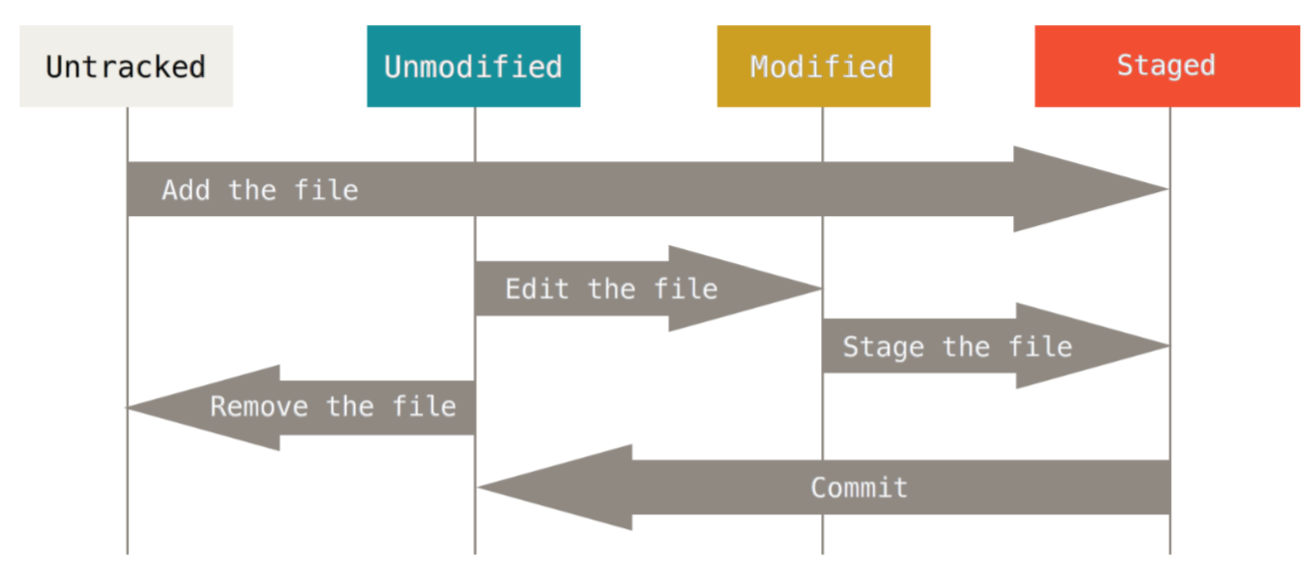
\includegraphics [width=1\textwidth]{image.png} 
\caption {\label{image} mon image}
\end{figure}
 \smallbreak
L'instruction \texttt{ \textbackslash begin {figure [!h]}} force l'image à se positionner comme on le désire. 
Le positionnement de l'image dépend également de ses dimensions, si elle est située en bas de page, et qu'elle est trop grande, elle va se positionner sur la page suivante et le texte qui suit se retrouvera donc avant l'image. Il faudra réduire la taille.
Ceci peut se faire avec l'option scale de \texttt{ includegraphics}.
\subsection {Sous titre 1}
\subsection {Sous titre 2}
\section {Partie 2- Les tableaux en Latex}
Les algorithmes de LaTeX pour mettre en forme les tableaux ont quelques imperfections. L'une d'entre elles est qu'il ne mettra pas automatiquement le texte sur plusieurs lignes dans les cellules, même si celui-ci déborde de la largeur de la page. Pour les colonnes qui contiendront une certaine quantité de texte, il est recommandé d'employer l'attribut p et d'indiquer la largeur désirée de la colonne (bien que cela puisse obliger à effectuer quelques ajustements avant d'obtenir le résultat escompté) (figure \ref{id-tab1} et figure \ref{id-tab2} ou figure \ref{id-tab3})\cite{x3} \cite{x4}.
\ldots
\begin{figure}[!h]
\begin{center}
\begin{tabular}{|l|c|r|}
\hline Un titre de colonne & Un autre titre & Un dernier \\
\hline à gauche & centré & à droite \\
\hline d & e & f \\
\hline Si j'écris plus de texte je dépasse la taille de la page &  texte &  texte\\
\hline
\end{tabular}
\end{center}
\caption{\textit{Un tableau simple}}\label{id-tab1}
\end{figure}

\begin{figure}[!h]
\begin{center}
\begin{tabular}{|l|p{2.5cm}|} \hline
   1 - 1 & Du texte  \\      \hline
   2 - 1 & On met un grand texte qui sera sur plusieurs lignes \\ \hline
\end{tabular}
\end{center}
\caption{\textit{Un autre tableau}}\label{id-tab2}
\end{figure}

\newcolumntype{M}[1]{>{\raggedright}m{#1}}
\begin{figure}[!h]
\begin{center}
\begin{tabular}{|l|M{5cm}|}
    \hline
    colonne 1 & colonne "M" \tabularnewline
    \hline
    court texte & Texte plus long qui sera centré dans la ligne et aligné à gauche dans la colonne \tabularnewline
    \hline
 \end{tabular}
 \end{center}
\caption{\textit{Un autre tableau bis }}\label{id-tab3}
\end{figure}

\section {....}
\section {Conclusion}


\section {Bibliographie} Veillez à citer les sources bibliographiques d'où vous extrayez des informations dans le coeur de votre article et les référencer explicitement dans cette partie. 
\ \\
Consultez les documents mis à disposition (Rédaction d'une biblio) pour la mise en forme de cette bibliographie (cf Normes APA) \cite{x1} 
\cite{x2}.

Vous pouvez utiliser un fichier .bib pour insérer votre bibliographie, et citer vos références de la manière suivante: \cite{greenwade93}

\begin{thebibliography} {99}
\bibitem[1]{x1} \url {https://www.scribbr.fr/category/normes-apa/}
\bibitem[2]{x2} \url {https://bib.umontreal.ca/citer/styles-bibliographiques/apa?tab=3281/}
\bibitem[3]{x3} \url
{https://fr.wikibooks.org/wiki/LaTeX/Tableaux}
\bibitem[3]{x4} \url{https://zestedesavoir.com/tutoriels/826/introduction-a-latex/1322_completer-vos-documents/images-tableaux-et-texte-preformate/#2-tableaux}
\end {thebibliography}


\bibliographystyle{alpha}
\bibliography{bib}



%The \Gls{latex} typesetting markup language is specially suitable for documents that include \gls{maths}. 

The \Gls{latex} typesetting markup language is specially suitable for documents that include \gls{maths}. \Glspl{formula} are rendered properly an easily once one gets used to the commands.

Given a set of numbers, there are elementary methods to compute its \acrlong{gcd}, which is abbreviated \acrshort{gcd}. This process is similar to that used for the \acrfull{lcm}.

%\clearpage

\printglossary

\section {Annexe}  Celles citées dans l'intro +  illustrations qui prendraient trop de place ou complètent les illustrations déjà insérées  - mais ne mettez pas toutes les illustrations en annexe  ! 
\end{document}
